\subsection{Overview}

Our S\&C subsystem consists of a 
\begin{itemize}
    \item Control Boards: \begin{itemize}
            \item Braking Controller
            \item Thermal (Cooling) Controller
    \end{itemize}

    \item Telemetry Device: \begin{itemize}
            \item CAN Bus
            \item Telemetry Transceiver
            \item Network Transceiver
            \item GUI/Logging system
    \end{itemize}
\end{itemize}
In this section, the main components of the sensor network and software architecture shall be described, as well as their basic functionality. A special focus shall be made on how safety mechanisms are implemented in these systems. Extensive design descriptions are expected for, if applicable:

\subsection{Control Boards}
\subsubsection{Introduction}
\begin{enumerate}
    \item Brief overview of all control boards (Brakes, Thermal)
    \item Diagram with the connection of all boards with NAP and control station.
    \item Brief description of communication protocols used.
\end{enumerate}

% Merged detailed content from the first snippet

\subsubsection{Parts Lists}
Example Thermal Partslist start:
% Comprehensive list of all parts used in the thermal system, including specifications and suppliers.
Parts list:
\begin{table}[h]
    \centering
    \caption{Parts List}
        \begin{adjustbox}{width=\textwidth,center}
    \begin{tabular}{|c|c|c|c|c|c|c|}
        \hline
        \textbf{Amount} & \textbf{Name} & \textbf{Company, (Serial Number)} & \textbf{Dimensions [mm x mm x mm]} & \textbf{Weight [kg]} & \textbf{Nominal Voltage} & \textbf{Expected max current} \\
        \hline
        32 & Additional Temperature Sensors (NTC, 10k Ohm) & Company & 2x2x2 & 0 & - & - \\
    \end{tabular}
        \end{adjustbox}
\end{table}


\subsection{State Machine of the Vehicle}
% Continue with the structured format from the second snippet, ensuring to merge relevant content from the first snippet into these sections.

Our states are different for each component.

\subsection{Code Architecture and Class Diagram}
% Insert content from the first snippet related to Code Architecture here.
For the brakes, we adhere to: \\

The software follow a simple state: \\
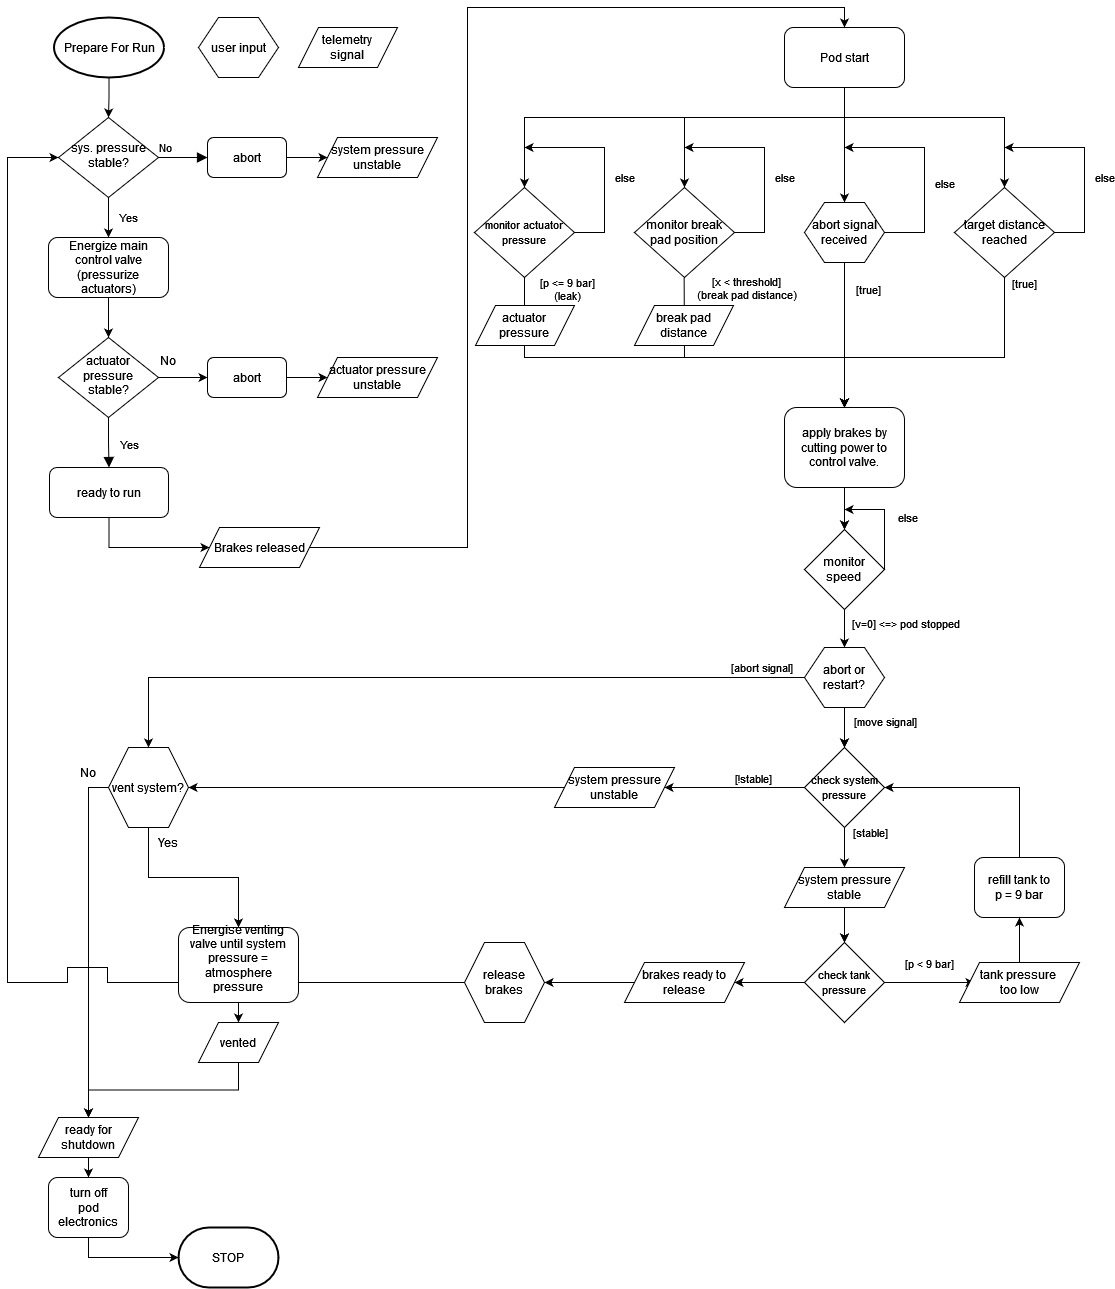
\includegraphics[width=\textwidth]{texfiles/elec/eimg/brakesoftware_ext}


\subsection{Control Boards/Units in the Vehicle}
% Insert content from the first snippet related to Control Boards/Units in the Vehicle here.

\subsection{Communication and Navigation}
% Insert content from the first snippet related to Communication and Navigation here.

\subsection{Integration with other systems}
The friction brakes, the cooling pump and the motor are controlled through our system.

\subsection{Graphical User Interface (GUI)}
% Insert content from the first snippet related to GUI here.

% Continue merging additional sections and sub-sections from the first snippet into the structured format of the second snippet as needed.
